\documentclass{beamer}

\mode<presentation>{
  \usetheme{Madrid}
}

\usepackage{graphicx}
\usepackage{booktabs}
\usepackage{tabularx}
\usepackage{graphicx}
\usepackage[sc]{mathpazo}
\usepackage[T1]{fontenc}
\usepackage[labelfont=sf,hypcap=false,format=hang,width=1\columnwidth]{caption}
\usepackage{longtable}
\usepackage{tabularx}
\usepackage{array}

\title[Project in STK-INF4000.]{Investigations of road traffic and delays on the railroad}
\author{Kristofer, Maria, Andr\'{e}, Jo\"{e}l}
\institute[UiO]{University of Oslo\medskip}
\date{\today}

\begin{document}

\begin{frame}
\titlepage
\end{frame}

%Suggested topics to talk about, and more in depth discussion are given in the comments after each frame/slide.

\begin{frame}
\frametitle{Project Goal}
%Model and  predict train delays and investigate the impact passenger train delays has on road traffic in and around Oslo.
\begin{itemize}
\item Model and predict train delays and road traffic
\item Investigate the relation between them 
\item In and around Oslo
\end{itemize}
\end{frame}
%Our goal 
%Model and predict train delays and Investigate the impact passenger train delays has on Road traffic in and around Oslo



%Sconcentrated on passenger train delays and road traffic, and the relation between them. And especially whether train delays would cause any increase in the number of cars on the roads. 

\begin{frame}
\frametitle{Motivation}
\begin{itemize}
%\item Problem in society
\item  Many  people rely on trains
\item  Changed travel behavior?
\item  Negative effect on the environment from car use 
\item Get from A to B efficiently 
\end{itemize}

%What is the motivation for that? 
%Well, a lot of people rely on trains in their daily lives and will be affected if trains are delayed.  If this happens frequently it might question the reliability of the railway system and might in turn change people's travel behavior. 
%There are also negative external effects on the environment with a lot of car use. 
%So to understand the factors that cause delays as well as the relation to the road traffic, if any, is therefore of great interest.

\end{frame}

\begin{frame}\frametitle{Potential business partners}
\begin{itemize}
\item Transport and Environment Department of Oslo kommune
\item Jernbaneverket and NSB
\item Taxi companies
%New
\item The public%(an app, webapp?)
\end{itemize}
\end{frame}
%App which compares traffic with train delays to suggest the best mode of transportation?

%\begin{frame}\frametitle{}
%\end{frame}

%It did not seem to be much of a link between them?
%Therefore made prediction models for both train delays and car traffic and compare the two by suggesting the best mode of transportation for a given day(and hour?).


\begin{frame}\frametitle{Datasets}
% Say something about what he asked about here.
% Outliers in train data? Weather data?
% ** coordinate data! **
\begin{itemize}
\item Weather Data
\item Train Data
\item Road traffic data
\end{itemize}

\end{frame}

\begin{frame}\frametitle{Datasets: Weather data}
%Datasets 1
\begin{itemize}
\item Scraped from the yr.no website's historical data using BeautifulSoup and regular expressions.
%\item Data: type of weather, temperature and wind speeds for every hour.
\item We used the Blindern weather station which had the most detailed data for the Oslo region.
\item Data gathered into MongoDB, then transformed to CSV.
%\item Only sporadic measurements for type of weather was given. We used nearest neighbor interpolation to fill in the gaps.
\end{itemize}
\end{frame}

\begin{frame}\frametitle{Datasets: Train data}
%Datasets 2
\begin{itemize}
\item SQLite database file received from Jernbaneverket.
\item One entry each time a train stops at a station, from 2012 to 2016.
\item When the train should have arrived, when it did arrive, and where.
\item Too large to handle directly, so we aggregated delay data per day and hour.
\end{itemize}
\end{frame}


\begin{frame}\frametitle{Datasets: Road traffic data}
%Datasets 3
\begin{itemize}
\item Received from Vegvesenet.
\item Hourly counts of number of cars passing in each lane of the road.
\item Twenty one different locations.
\item Also counts by car length categories.
%\item Somewhat fiddly due to Excel format, and gaps in the data.
%\item E.g. all of 2014 missing for Maritim.
\end{itemize}
\end{frame}

\begin{frame}\frametitle{Map of counting points}
\begin{figure}
\includegraphics[width=0.55\textwidth]{map_oslo_tellepunkt_modif.png}
\caption {Road traffic measurement points.}
\end{figure}
\end{frame}




% Her kommer bubble plot


\begin{frame}\frametitle {Bubble plot of train delay. }
\begin{figure}
  \centering
  \includegraphics[width=0.95\textwidth]{bublleeeeee.jpeg}
 \end{figure}
\end{frame}

% Her we have bubbles plots of the mean delay versus their spatial coordinates.The size of the dots are proportional to the value of the mean delay. Visual inspection shows no strong pattern in the distribution of the delay. We observe that the size of the dots are randomly distributed.

\begin{frame}\frametitle{Train delay data}
\begin{figure}
  \centering
   \includegraphics[width=0.75\textwidth]{plots/delay2log-crop.pdf}
    \caption{Distribution of train delay on the whole network.}
\end{figure}
\end{frame}

% \begin{frame}\frametitle{Train delays}
% \end{frame}
%Initially looked at a link between type of weather and historical data in order to predict number of train delays for a given hour. Train delays were categorized in 4 categories: 2 to 3, 3 to 5 , 5 to 10, 10 to 20 minutes. This worked somewhat well, but there was some problems, especially with predicting peaks.
%Updated model looks at the different lines and directions instead of the whole network. It predicts average minutes delayed for a given line, instead of number of trains delayed on the whole network.

%Had to perform a lot of data manipulation in order to extract the lines and direction of each train.
%In addition we wanted the delay given by the time difference between scheduled departure time and actual departure of the next train leaving the station. We therefore had to find the next train leaving from the station, which did not turn out to be a trivial task.

\begin{frame}\frametitle{Predicting road traffic from train delays}
\begin{itemize}
\item Recap: Try to predict road traffic at certain detectors ("counting positions").
\item I found that median daily train delays weren't useful, but time of year was.
\item But what about using only train delay data from stations near the road in question?
\item I started doing this, which entailed quite a bit of aggregation work.
\item First attempt: mean of train delays among closest four stations, for each counting point
% Why didn't the first attempt work?
% Things to point out: more robust to outliers, 1 train at 20min delay is not the same
% thing as 10 trains at 2 min delay each.
\item Second attempt: number of delays in intervals [-2...0) hrs, [0...1) min, [1...5), [5...15), [15...$\infty$), as well as number of cancellations. Lower AIC.
\end{itemize}
\end{frame}

\begin{frame}\frametitle{Predicting road traffic from train delays}
\begin{itemize}
\item Counted the number of delays in total for each interval for all train stations within 8 km
\item Final models found by thinking and using subset selection:
\begin{itemize}
\item Baseline model: same as in midterm (only weekday, month, holiday, easter effects)
\item Model with weather: Baseline, plus amount of snow in the day in question, weather type, middle temperature
\item Full model: Model with weather, plus number of delays within 8 km
\end{itemize}
\item Fitted model to 2012-2015 and predicted for 2016.
% Mention actual RMSEs here.
\item Weather model much lower RMSE than baseline (5860 vs 6210)
\item Full model had worse RMSE than both at 6450
\item But likelihood ratio test shows significance between full and weather-only models with better likelihood for the full model
\end{itemize}
\end{frame}

\begin{frame}\frametitle{Traffic prediction, plot 1}
\begin{figure}
  \centering
   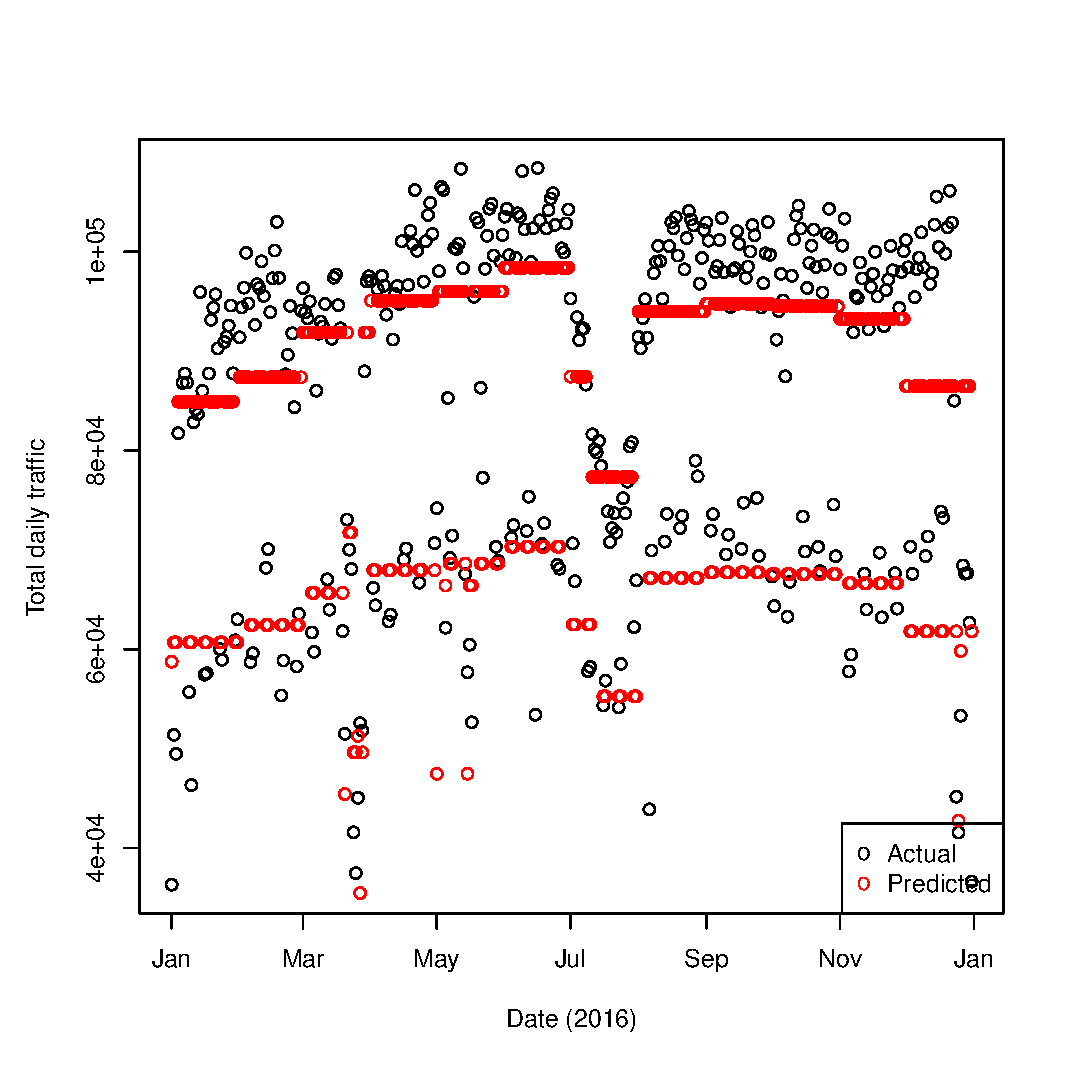
\includegraphics[scale=0.35]{plots/predict_maritim_dateonly.eps}
    \caption{\textbf{Predicted and actual traffic for Maritim 250B, \hspace{\textwidth}base model}}
\end{figure}
\end{frame}

\begin{frame}\frametitle{Traffic prediction, plot 2}
\begin{figure}
  \centering
   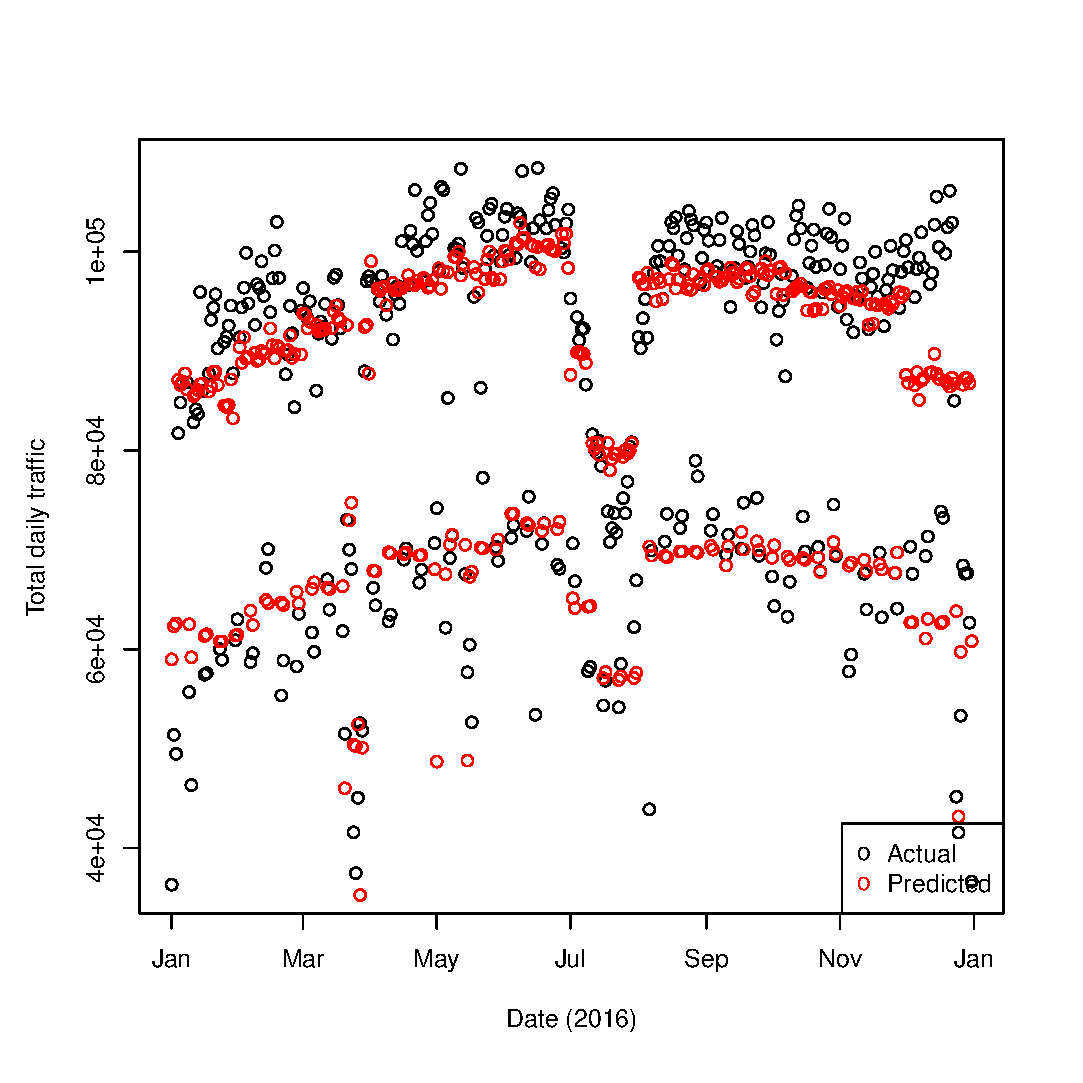
\includegraphics[scale=0.35]{plots/predict_maritim_withweather.eps}
    \caption{\textbf{Predicted and actual traffic for Maritim 250B, \hspace{\textwidth}weather model}}
\end{figure}
\end{frame}

\begin{frame}\frametitle{Traffic prediction, plot 3}
\begin{figure}
  \centering
   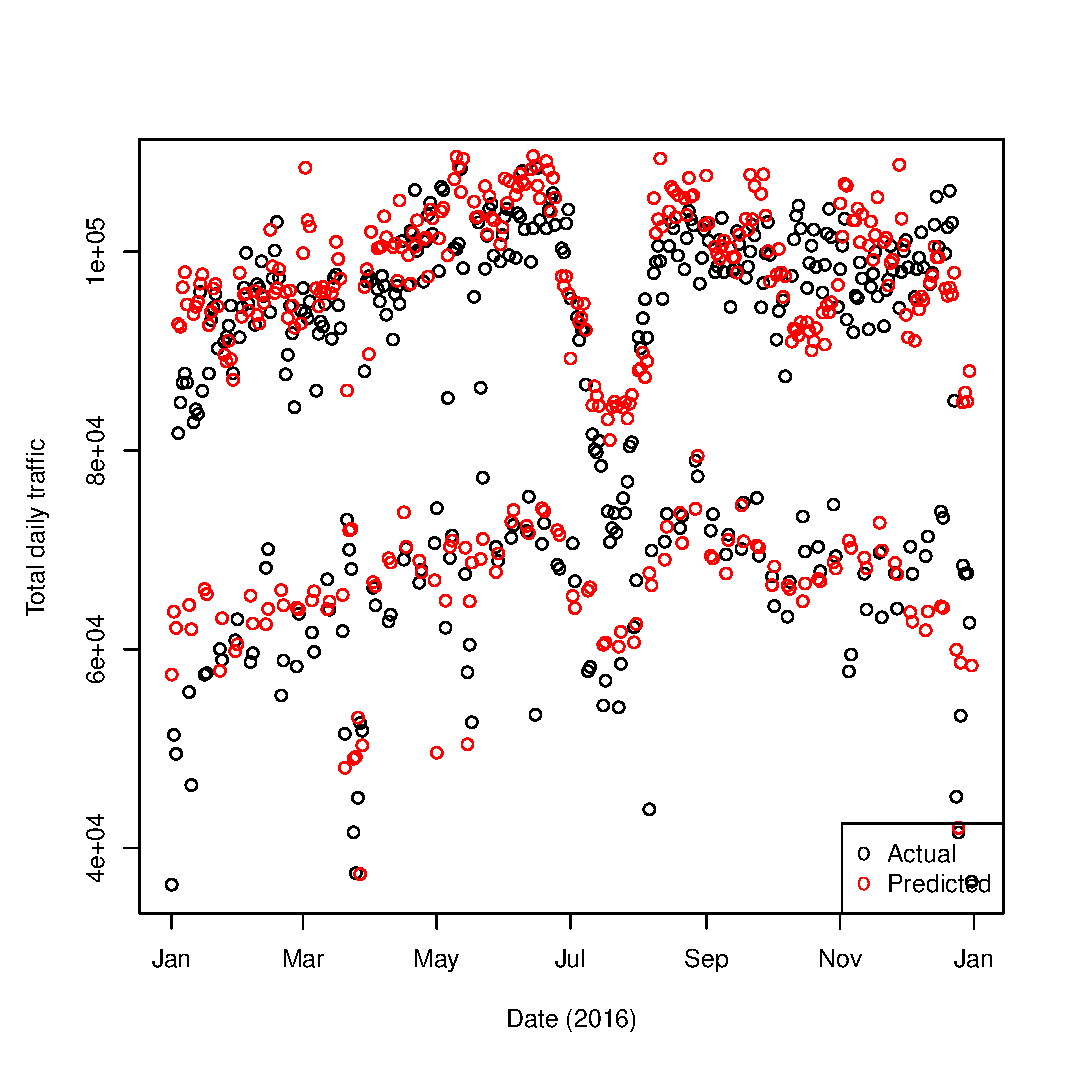
\includegraphics[scale=0.35]{plots/predict_maritim_everything.eps}
    \caption{\textbf{Predicted and actual traffic for Maritim 250B, \hspace{\textwidth}full model}}
\end{figure}
\end{frame}

\begin{frame}\frametitle{Predicting road traffic from train delays}
\begin{itemize}
\item Small effects
\begin{itemize}
\item One additional cancellation: 0.033\% increase in traffic.
\item In contrast: Weekend: 27\% reduction compared to weekdays
\end{itemize}
\item Possible reasons
\begin{itemize}
\item Roads have finite capacity (traffic jams).
\item Time lag?
\end{itemize}
\item Difficult to use the model for prediction when the effects are small.
\item Easier with large effects like weather and holidays!
\end{itemize}
\end{frame}

\begin{frame}\frametitle{Predicting delays on the railway}
\begin{itemize}
\item Predicting delays within zone 2.
\item Predicting average number of minutes delayed.
\item Hourly prediction.
\item Splitting the network into 6 groups.
\end{itemize}
\end{frame}

\begin{frame}{Train line map}
\begin{figure}
  \centering
   \includegraphics[width=1.0\textwidth]{plots/linjekart-crop.pdf}
    \caption{Visualization of train lines in the Oslo region. Lines are categorized into three main branches.}
\end{figure}
\end{frame}

% \begin{frame}\frametitle{Correlation between lines}
% \begin{table}
% \begin{center}
% \Large
% \begin{tabular}{|c||c|c|c|c|c|c|}\hline
% Lines & 1 w & 1 e  & 2 w  & 2 e  & 3 w  & 3 e \\\hline\hline
% 1 west& 1.00&  0.37&  0.18&  0.63&  0.42& 0.15\\\hline
% 1 east& 0.37&  1.00&  0.16&  0.36&  0.37& 0.12\\\hline
% 2 west& 0.18&  0.16&  1.00&  0.15&  0.14& 0.58\\\hline
% 2 east& 0.63&  0.36&  0.15&  1.00&  0.38& 0.14\\\hline
% 3 west& 0.42&  0.37&  0.14&  0.38&  1.00& 0.11\\\hline
% 3 east& 0.15&  0.12&  0.58&  0.14&  0.11& 1.00\\\hline
% \end{tabular}
% \normalsize
% \end{center}
% \caption{Correlation of delay between all train lines and directions.}
% \end{table}
% \end{frame}
%Seems to be some correlation between lines 1w and 2e, and 2w and 3e. But mainly low correlation.
%Treating the lines as separate entities is probably justifiable, and a decent approximation?

\begin{frame}\frametitle{Finding delay till next train}
\begin{itemize}
\item $2/3$ of the trains in the data have line numbers.
\item Increased number to $91\%$, by matching visiting stations with lines.
\item Direction is found by which order trains visits the stations.
\item Finds delay till next train arrives at a station, if a train is delayed.
\end{itemize}
\end{frame}


\begin{frame}\frametitle{Train delay prediction model}
\begin{itemize}
\item Tried two models: Gradient boosted decision trees and neural network.
\item Training on data from 2012 to 2015 and testing on 2016.
\item Input data:
	\begin{itemize}
    \item One hot encoded weather data.
    \item Historical data periodicities: 1 hour, 1 day and 1 week.
    \item Historical data: max and mean delay, number of trains. 
    \end{itemize}
\end{itemize}
\end{frame}

\begin{frame}\frametitle{Decision trees vs. neural networks}
\begin{table}
\begin{center}
\Large
\begin{tabular}{|c||c|c|c|c|c|c|}\hline
Model & 1 w & 1 e  & 2 w  & 2 e  & 3 w  & 3 e \\\hline\hline
MLP& 606&  455&  410&  404&  512& 337\\\hline
GBT& 605&  473&  417&  410&  518& 337\\\hline
\end{tabular}
\caption{$L_2$ norm of the error(in minutes) of testing data for a multilayered perceptron model and a gradient boosted tree model.}
\normalsize
\end{center}
\end{table}
\end{frame}

\begin{frame}\frametitle{Prediction of train delays}
\begin{figure}
  \centering
   \includegraphics[width=0.5\textwidth]{plots/1w-crop.pdf}
   \includegraphics[width=0.5\textwidth]{plots/1wt-crop.pdf}
    \caption{Predicted delay vs. measured data for line 1 heading west. Neural network to the left and gradient boosted trees on the right.}
\end{figure}
\end{frame}

\begin{frame}\frametitle{Did we meet our goals?}
\begin{itemize}
\item Models to predict train delays
\item Models to predict  road traffic
\item Investigated the impact of train delays on road traffic
\item Compare the two models to suggest mode of transportation
\end{itemize}
\end{frame}

\begin{frame}
\begin{center}
\Large Thank you!
\end{center}
\end{frame}

%\begin{frame}\frametitle{Prediction error.}
%\begin{figure}
%  \centering
%   \includegraphics[width=0.5\textwidth]{plots/1we-crop.pdf}
%   \includegraphics[width=0.5\textwidth]{plots/1wet-crop.pdf}
%    \caption{Error distribution of the prediction of train delays on line 1 heading west. Neural network to the left and gradient boosted trees on the right.}
%\end{figure}
%\end{frame}











\end{document}